\chapter{Desarrollo}
\section*{Introducci'on}

En 'este cap'itulo se muestra la arquitectura de los distintos esquemas de calendarizaci'on de trabajos en un entorno en la nube, para la implementaci'on de dichos esquemas se hace uso de un framework llamado CloudSim, el cual será definido de igual manera.





\addcontentsline{toc}{section}{Introducci'on}
\section{Aplicaci'on del marco metodol'ogico y de actividades de experimentaci'on}

En base de los dos primeros puntos descritos anteriormente en el marco metodol'ogico se realizar'on las siguientes activides:

\begin{itemize}
	\item \textbf{Simular:} Se implementar'a a manera de simulaci'on un centro de datos con un entorno en la nube, las m'aquinas virtuales y el servidor inicializador que lo conforman.
	\item \textbf{Implementar:} En el centro de datos se desarrollar'an los algoritmos de calendarizaci'on que se mencionan con antelaci'on.
\end{itemize}

\subsection{Simulaci'on del Centro de Datos en la Nube}

 \textbf{Cloudsim} es un nuevo, generalizado y extensible framework de simulaci'on, que permite el modelaje, simulaci'on y experimentaci'on de infraestructuras emergentes de c'omputo en la nube y servicios de aplicaci'on (\citeauthor{calheiros2011cloudsim}, \citeyear{calheiros2011cloudsim}, p. 2).

Entre los componentes que proporciona dicho framework se encuentran los siguientes:

\begin{itemize}
	\item  \textbf{Cloudlet:} Esta clase modela las aplicaciones de servicio basadas en la nube como pueden ser env'io de contenido, redes sociales, y flujo de trabajo empresarial (\citeauthor{calheiros2011cloudsim}, \citeyear{calheiros2011cloudsim}, cap. 4).
	\item  \textbf{Datacenter:} Esta clase modela el nucleo de los servicios en un nivel de infraestructura (hardware) que son ofrecidos por Cloud Providers (Amazon, Azure, App Engine). Estos son encapsulados en un conjunto de host que pueden ser homogeneos o heterogeneos con respecto a sus configuraciones de hardware (memoria, n'ucleos, capacidad, y almacenamiento) (\citeauthor{calheiros2011cloudsim}, \citeyear{calheiros2011cloudsim}, cap. 4).
	\item  \textbf{DatacenterBroker:} Esta clase modela un broker, el cual es responsable de mediar las negociaciones entre el SaaS y los Cloud providers; y dichas negociaciones son manejadas por los requerimientos QoS (\citeauthor{calheiros2011cloudsim}, \citeyear{calheiros2011cloudsim}, cap. 4).
	\item  \textbf{Host:} Esta clase modela los recursos f'isicos como una computadora o un servidor de almacenamiento (\citeauthor{calheiros2011cloudsim}, \citeyear{calheiros2011cloudsim}, cap. 4).
	\item  \textbf{Vm:} Esta clase modela una M'aquina Virtual (VM), la cual es administrada y hosteada por un componente host en la nube. Cada VM tiene acceso a un componente que almacena las siguientes características relacionadas a una VM: memoria accesible, procesador, tama'no de almacenamiento (\citeauthor{calheiros2011cloudsim}, \citeyear{calheiros2011cloudsim}, cap. 4).
\end{itemize}



\begin{figure}
	\caption{Estilo de Trabajo de CloudSim, Fuente: Chatterjee et al.}
	\centering
	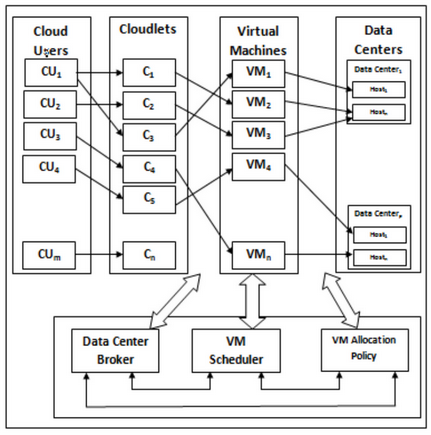
\includegraphics[scale=0.5]{media/imagenuno}
\end{figure}


\subsection{Implementaci'on de los Algoritmos}

Existen varios algoritmos para calendarizar los trabajos en el c'omputo en la nube. La mayor ventaja de estos algoritmos es obtener el mayor rendimiento. Los principales ejemplos de algoritmos de calendarizaci'on son: FCFS, Round Robin, Min-Min, Max-Min y algoritmos de meta heurísticas  (\citeauthor{shimpy2014different}, \citeyear{shimpy2014different}, p. 1).



De los algoritmos mencionados anteriormente, se presentan los siguientes:


\begin{itemize}
	\item  \textbf{FCFS:} Ejecuta las tareas en orden de llegada, es decir, el primero en llegar es el primero en ser atendido.
	\item  \textbf{Min-Min:} Selecciona las tareas m'as pequeñas para ser ejecutadas primero.
	\item  \textbf{Max-Min:} Selecciona las tareas m'as grandes para ser ejecutadas primero.
\end{itemize}

En un entorno de trabajo normal, la forma descrita anteriormente la podemos ver de la siguiente manera:

\begin{figure}
	\caption{Esquema de trabajo de algoritmos de calendarizaci'on
		Fuente: Elaboraci'on propia.}
	\centering
	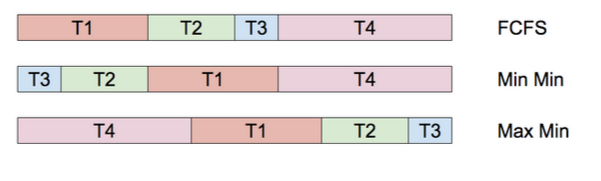
\includegraphics[scale=0.5]{media/imagendos}
\end{figure}


\newpage
Sin embargo en un entorno en la nube, al ser m'ultiples m'aquinas virtuales alojadas en distintos hosts, que a su vez pueden formar parte de uno o m'as datacenters, dicho esquema tiene que ser adaptado para poder adoptar un estilo de trabajo similar al proporcionado por el framework, por lo que los resultados quedan de la distinta manera:

\begin{figure}
	\caption{Arquitectura FCFS para un entorno en la nube. Fuente: Elaboraci'on propia.}
	\centering
	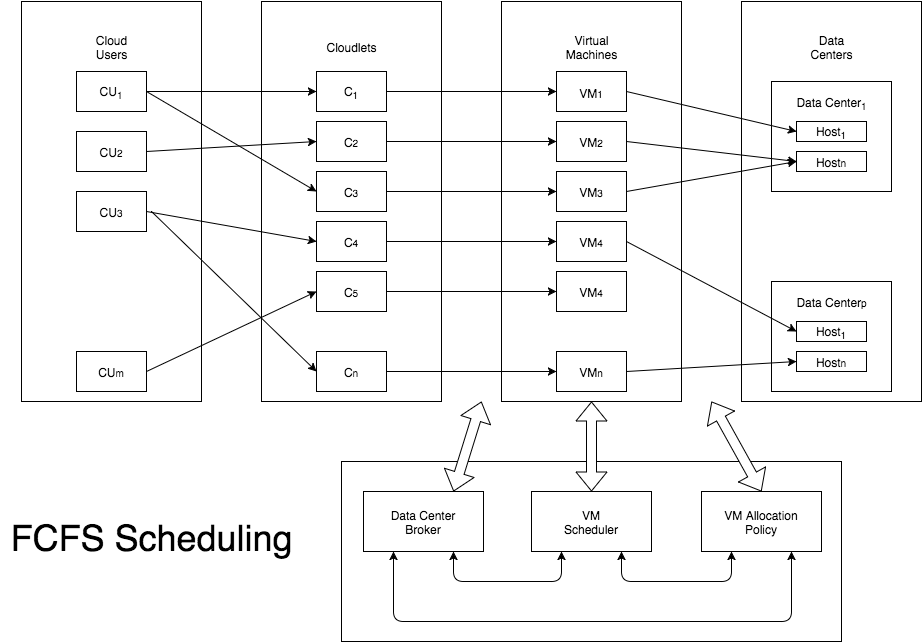
\includegraphics[scale=0.5]{media/imagentres}
\end{figure}



Como podemos apreciar en el diagrama, podemos tener \emph{m} usuarios ejecutando \emph{n} tareas, sin embargo la asignaci'on de m'aquinas virtuales va dependiendo del orden de llegada de dichas tareas, y quien se encarga de repartir las tareas es el datacenterBroker.

De manera similar tenemos los siguientes algoritmos min-min y max-min:



\begin{figure}
	\caption{Arquitectura de Max-Min para un entorno en la nube. Fuente: Elaboraci'on propia.}
	\centering
	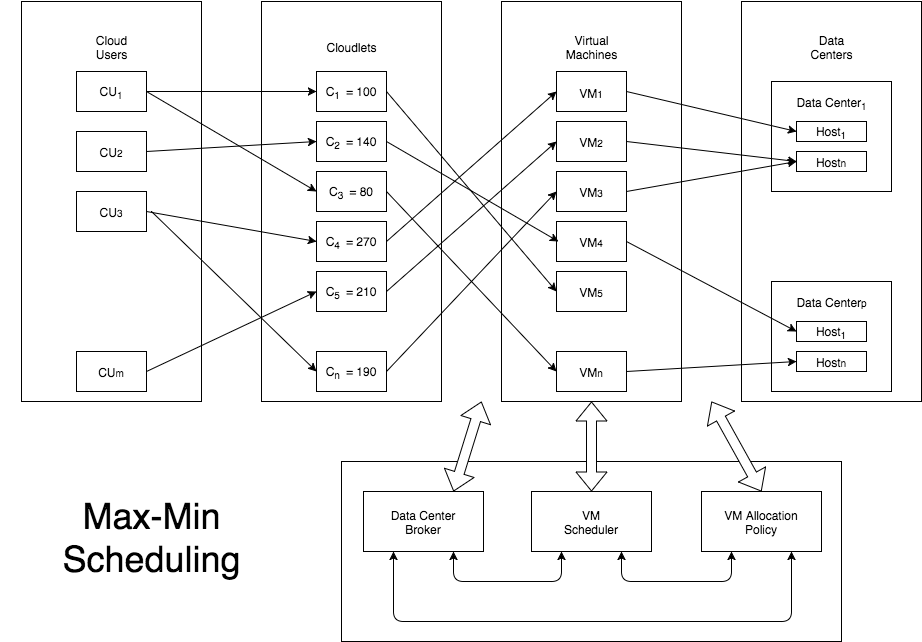
\includegraphics[scale=0.5]{media/imagencuatro}
\end{figure}


\begin{figure}
	\caption{Arquitectura de Min-Min para un entorno en la nube. Fuente: Elaboraci'on propia.}
	\centering
	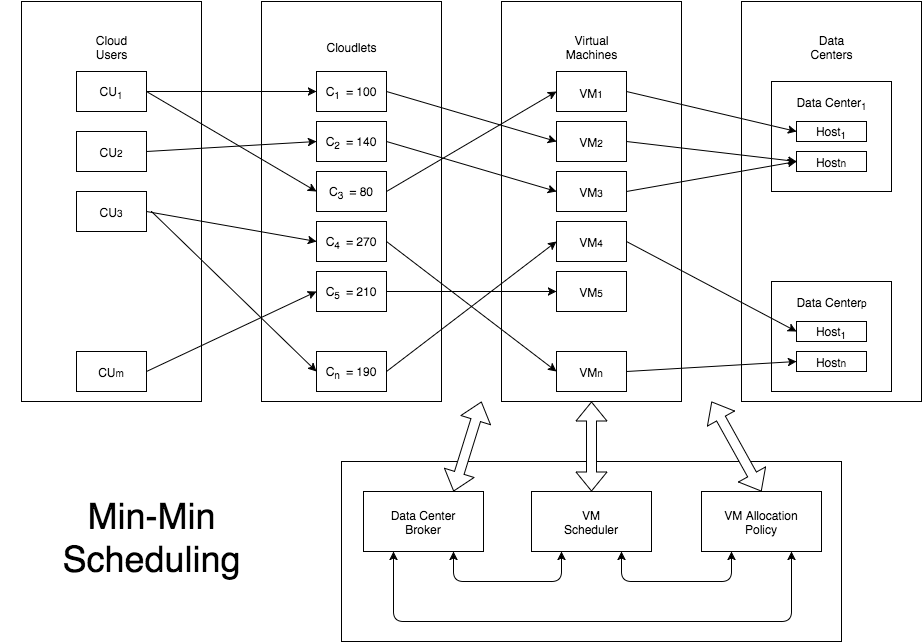
\includegraphics[scale=0.5]{media/imagencinco}
\end{figure}

\newpage
Est'as son algunas capturas del c'odigo para la implementaci'on de los primeros algoritmos, el centro de datos:

%ver la seccion anexo